\documentclass[prd,10pt]{revtex4-2}

\usepackage{amsmath,amssymb,graphicx,color,microtype,physics,hyperref}
% Remove the 'footnote' package
% \usepackage{footnote}

\usepackage{CJK}
\bibliographystyle{apsrev4-2}

\begin{document}

\numberwithin{equation}{section}

\begin{CJK*}{GB}{}
    \title{GRB Note}
    \date{\today}
    \author{Lingyu Xia}
    \maketitle
\end{CJK*}



\tableofcontents


\section{Introduction}

Gamma-ray bursts (GRBs) are among the most violent and high-energy stellar explosions in the universe. They are believed to originate from the death of massive stars—particularly those whose bursts last longer than 2 seconds, often associated with a special class of supernovae—or from the merger of binary compact star systems, such as binary neutron stars. These mergers, which occur on very short time scales, can produce gamma-ray bursts lasting less than 2 seconds and are frequently linked to supernovae. Since the launch of the Fermi Gamma-ray Space Telescope in 2008, which operates in the 8 keV to 300 GeV range, significant advances have been made in the study of transient and high-energy radiation from gamma-ray bursts. In recent years, our understanding of GRBs has greatly improved due to new instruments, advanced analysis methods, and innovative ideas. The Power Density Spectrum (PDS) is a statistical tool used to analyze time series data, such as the light curves of GRBs. It illustrates how the power (or variance) of a signal is distributed across different frequency components. Essentially, the PDS helps identify and quantify periodicities, quasi-periodicities, and stochastic (random) variations in the light curves of GRBs. 

This article discusses the principles of the Power Density Spectrum (PDS) in the context of GRBs and explores the potential relationships between PDS and the mechanisms driving GRBs.

\section{Power Density Spectrum}
\subsection{Definition}
The PSD defines the amount of variability 'power' as a function of temporal frequency\cite{10.1046/j.1365-2966.2003.07042.x}. It is estimated by calculating the periodogram.

For an evenly sampled light curve (with a sampling period $\Delta T$) the periodogram is the modulus-squared of the discrete Fourier transform (DFT) of the data. For a light curve comprising a series of fluxes xi measured at discrete times $t_{i} (i = 1, 2, . . . , N )$:
We firstly introduce that how to calculate the power density spectrum. For a series of signal $x_{i}(t)$, we firstly take Fourier transformation

\begin{align}
    \hat{x}(f)=\int^{\infty}_{-\infty}  e^{-i2\pi f t}x(t)dt,
\end{align}
then we define the \textbf{energy spectral density}
\begin{align}
    \bar{S}_{x x} \equiv |\hat{x}(f)|^{2}.
\end{align} 
Also, for discrete-time signal, we have
\begin{align}
    \bar{S}_{x x}(f)=\lim_{N\rightarrow \infty}(\Delta t)^{2}\left|\sum_{n=-N}^{N}x_{n}e^{-2\pi fn\Delta t}\right|^{2},
\end{align}
at $N/2$ evenly spaced frequencies $f_{j}= j/N \Delta T$ (where $j = 1, 2,\cdots , N /2$), $f_{N/2} = 1/2 \Delta T$ is the Nyquist frequency, $f_{Nyq}$. Note that it is customary to subtract the mean flux from the light curve before calculating the DFT. This eliminates the zero-frequency power. The periodogram, $P( f_{j})$, is then calculated by choosing an appropriate normalization A. For example,

\begin{align}
    P(f_{i})=A\abs{\text{DFT}(f_{j})}^{2}=\frac{2\Delta T}{N}\abs{\text{DFT}(f_{j})}^{2}\label{DFT}.
\end{align}

If the time series is a photon counting signal such as normally encountered in X-ray astronomy, and is binned into intervals of T, the effect of Poisson noise is to add an approximately constant amount of power to the periodogram at all frequencies. With the above normalization this constant Poisson noise level is $2 \bar{x}$ (assuming the light curve is not background subtracted).

\begin{figure}[ht]
    \centering
    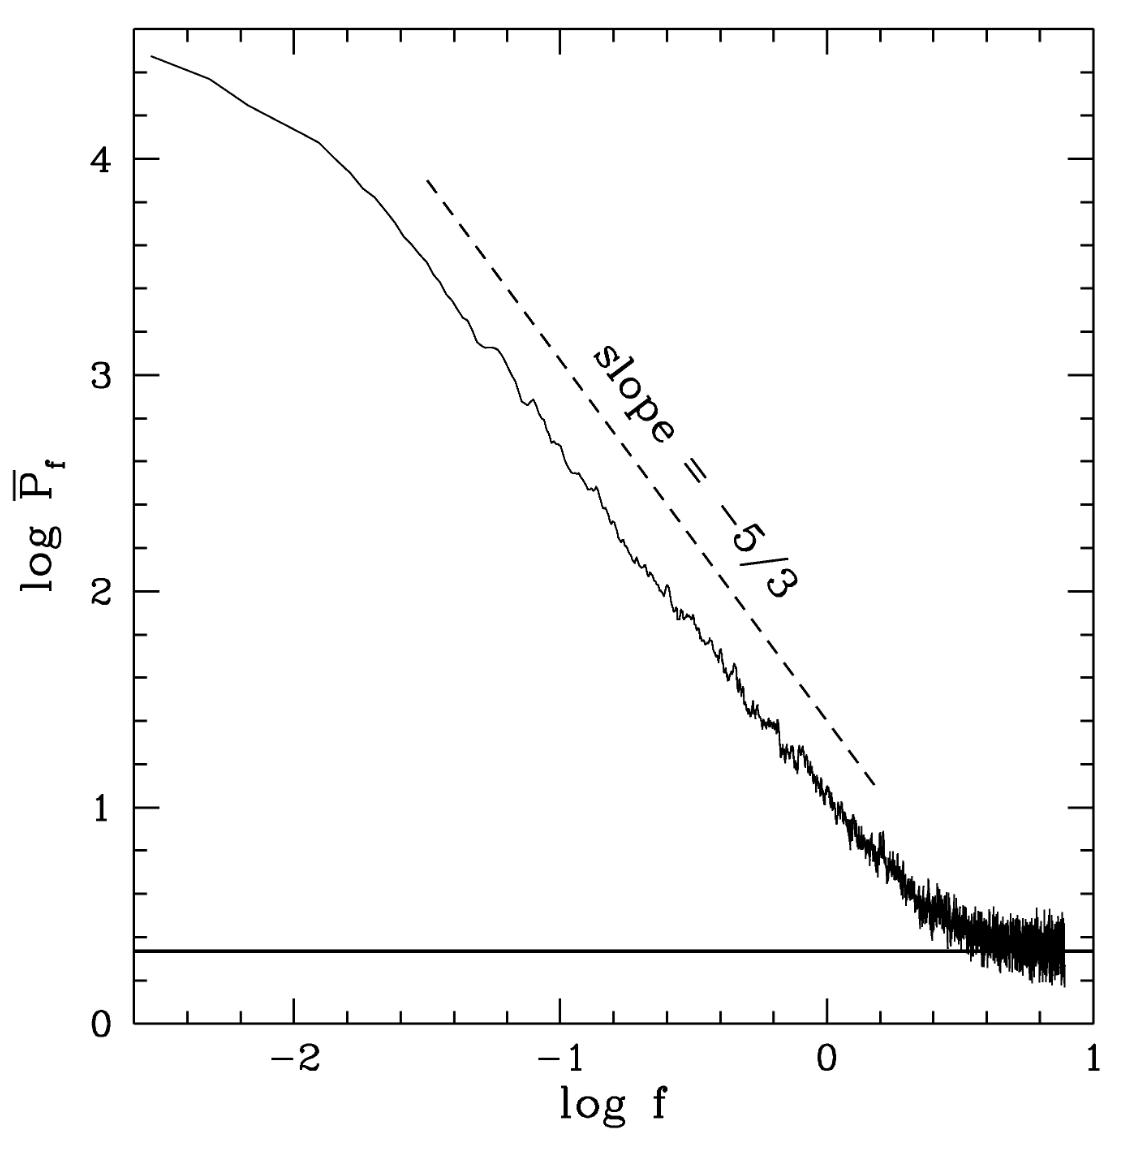
\includegraphics[width= 0.5\textwidth]{1.png}
    \caption{\label{fig:1.png}
        Power density spectrum's slope is around $-5/3$.\cite{Beloborodov:1998ai}.
    }
\end{figure}

\subsection{Motivation}

From Beloborodov's work \cite{Beloborodov:1998ai}, we start to use Fourier transformation to research GRB's properties. At first, we need to figure out why we should use the Power Density Spectrum (PDS). Here we list some points to explain the benefits of using PDS:

\begin{itemize}
    \item PDS is suitable for transients (\textbf{pulse-like} signals) whose energy is concentrated around one time window, which corresponds to the GRB. This concentrated energy distribution means that the signal exhibits a clear and distinct structure in the time domain, typically characterized by rapid rises and falls in intensity. These features make it straightforward to perform a Fourier transformation on the GRB signal, as the transformation can effectively capture the dominant frequencies and temporal characteristics of the burst. By converting the time-domain signal into the frequency domain, the PDS provides a powerful tool for analyzing the spectral properties of GRBs, allowing researchers to identify key frequencies and patterns that may be indicative of the physical processes driving the bursts. This method facilitates the study of transient phenomena by breaking down complex signals into more manageable components, highlighting periodicities, and distinguishing between different types of variations within the data.
    \item Noise discrimination: Background noise tends to be Gaussian, manifesting as white noise in the PDS, characterized by a flat spectrum with equal intensity across all frequencies. In contrast, real signals from GRBs often exhibit characteristic "red noise" behavior, where the power decreases with increasing frequency. This difference allows the PDS to effectively distinguish between genuine variations and random noise. By examining the PDS, researchers can identify and isolate the GRB signal from the background noise, ensuring that the observed variations are truly associated with the GRB event rather than random fluctuations. This noise discrimination capability is crucial for accurately analyzing and interpreting the data, as it enhances the signal-to-noise ratio and improves the reliability of the findings.
    \item Identify periodic signals: Very low-frequency features in the PDS may reveal periodic or quasiperiodic signals that provide clues about the central engine. These signals would be difficult to detect directly in the light curve.
\end{itemize}

For this article, we want to discuss whether PDS is related to the energy spectrum type of GRB, so as to explore the potential mechanism. We already know that the size of the fit slope of the energy spectrum is related to the type of GRB \cite{ghirlanda_extremely_2003}


\section{Processing the Signals}

\subsection{Extra Data}

To better know the relation between PDS and the mechanisms driving GRBs, we select several GRBs with known type of energy spectrum(Thermal or Non-thermal)

\subsection{Processing the Data}

To process the GRB's (time-series) photon counting signals, we have the following several modules to process the signals. Background analysis module, Significance calculation module, Light curve analysis module and Discrete Fourier transform module. The important computing modules are described below.

(1) Background analysis module

This module uses side bands method to estimate background. We select the background range around the gamma burst signal, and select the background range as the side bands. Multinomial equation of a certain order is selected as the background function model, and the background shape of side bands region is fitted with the least square method to estimate the background shape under the source signal in the counting energy spectrum. For example, in FIG. \ref{fig:bg.png} we select both ends of the background fragments before and after GRB signal, and perform polynomial fitting on them, and obtain the corresponding background fitting curve by using the least square method.

\begin{figure}[ht]
    \centering
    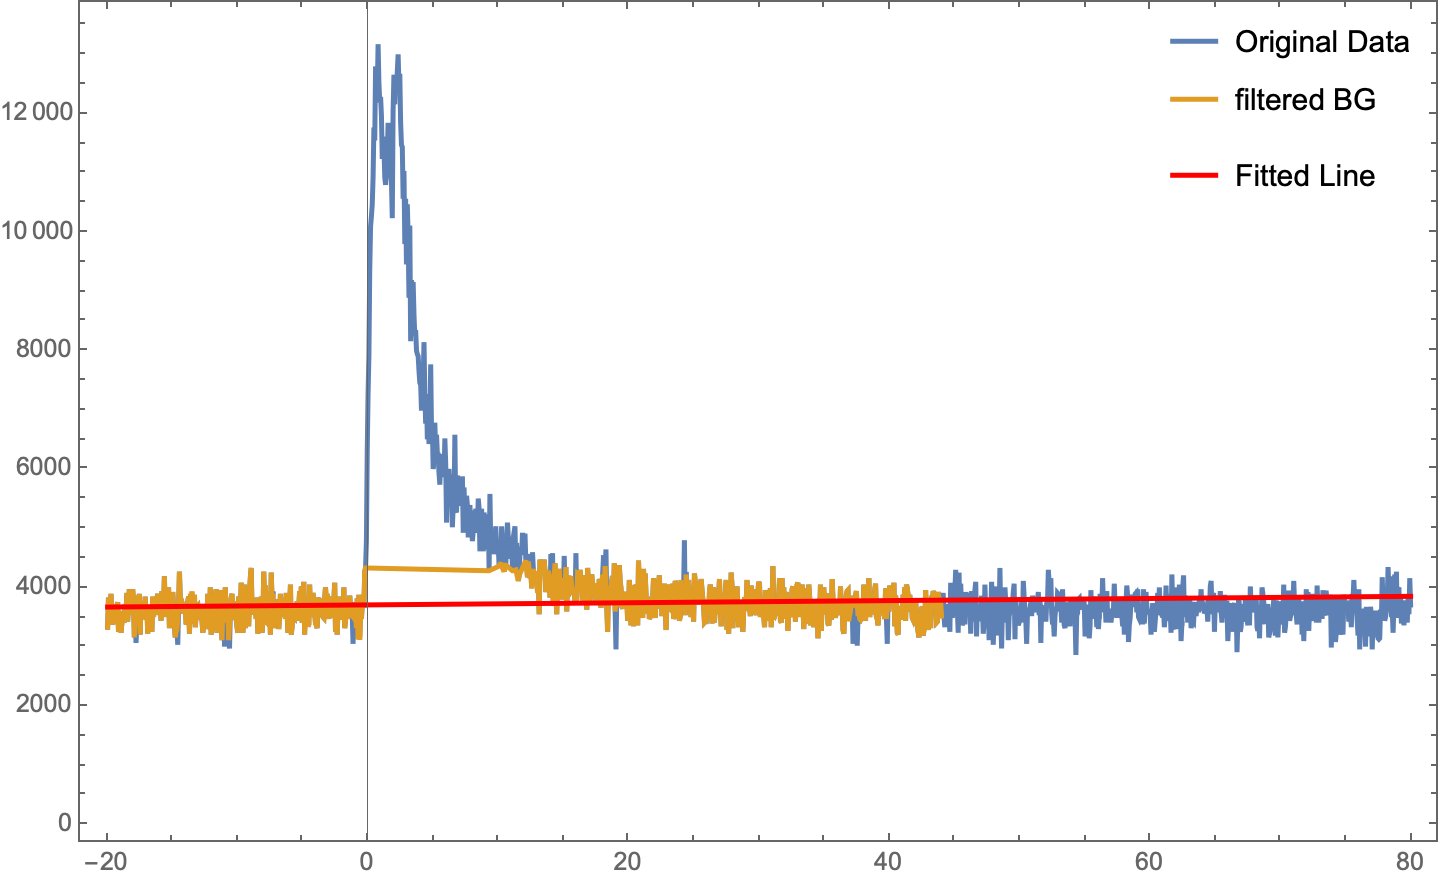
\includegraphics[width= 0.8\textwidth]{bg.png}
    \caption{\label{fig:bg.png}
        We have selected background range around the GRB, and fit background curve for  GRB110721200 in Fermi.
    }
\end{figure}

(2) Significance calculation module

For this part, assume that the background number $b$(obtained from the background analysis results) of each detector in the given signal interval and the total number of observed cases in the given signal interval are nobs, and the signal number is $s=n_{obs}-b$. The statistical significance (Sigma) of the source and the probability P-value of no signal in the signal region are calculated based on the B-value. When b is less than 25, the distribution of b conforms to the Poisson distribution law. The Poisson distribution is added to the experimental P-value, which is calculated as follows:
\begin{align}
    P&=P(n>n_{obs}|H_{0})\\
    &=\sum_{n=n_{obs}}^{\infty}f(n;s=0,b)\\
    &=1-\sum_{n=0}^{n_{obs}-1}\frac{b^{n}}{n!}e^{-b}
\end{align}

Where, $H_{0}$ is the assumption that there is no signal in the signal region. From $Sigma=s/\sqrt{b}$, the corresponding statistical significance was calculated. When $b$ is greater than 25, we consider that the Poisson distribution with large expected value is approximately Gaussian distribution, and the probability of the base number being $b$ under the no-signal hypothesis is calculated with Gaussian distribution, that is, the P-value. The corresponding statistical significance value (Sigma) defined by the P-value is as follows:
\begin{align}
    \int_{\text{Sigma}}^{-\text{Sigma}}\frac{1}{\sqrt{2\pi}}e^{-x^{2}/2}\dd{x}=1-P
\end{align}

The smaller the P-value, the greater the signal significance, that is, the greater the probability that there is a gamma burst source signal in the data.

(3) Light curve analysis module

For this part, we need to calculate GRB event duration $T_{90}$ and its error. $S$ is denoted as the integral of the number of instances of gamma burst signal observed at any time. $\tau_{f}$ is denoted as the time from the beginning point of time until $S$ reaches the $S_{\text{tot}}$ percentage of the total integral $f(\%)$.
\begin{align}
    \frac{f}{100}=\frac{\int_{\tau_{f}}^{\tau_{s}}(\dd{S}/\dd{t})\dd{t}}{S_{\text{tot}}}
\end{align}

The two characteristic quantities $T_{90}$ and $T_{50}$ marking the duration of gamma-ray bursts are defined by above equation as $T_{90}=\tau_{95}-\tau_{5}$ and $T_{50}=\tau_{75}-\tau_{25}$. The calculation method for the statistical error of T90 and T50 is given in reference \cite{1996ApJ...463..570K}.

\begin{align}
    & \left(\mathrm{d} S_f\right)_{\mathrm{cnt}}^2=\sum_{j=\tau_0}^{\tau_f}\left[\frac{\Delta C\left(t_j\right)}{\Delta t_j}\right] \Delta t_j, \\ & \left(\mathrm{~d} S_f\right)_{\text {fluc }}=\sqrt{\left(\frac{\partial S_f}{\partial L_0}\right)^2 \mathrm{~d} L_0^2+\left(\frac{\partial S_f}{\partial L_t}\right)^2 \mathrm{~d} L_t{ }^2 .}
\end{align}

It consists of two independent errors, which are the errors caused by the count of the starting point $\tau_{0}$ and the ending point $\tau_{t}(\Delta C(t))$, both of which are caused by the background. The statistical fluctuation is determined by the integral of the background over time. The total error is given by:
\begin{align}
    (\dd{S_{f}})_{\text{tot}}=\sqrt{(\dd{S_{f}})^{2}_{\text{cnt}}+(\dd{S_{f}})^{2}_{fluc}}.
\end{align}

(4)Discrete Fourier transform module

After we have determined T90, we can perform Fourier transform on the GRB light curve. Since the data is discrete data with a time interval of 64ms, we use the discrete Fourier transform expression of Eq. \ref{DFT}.
\begin{align}
    P(f_{i})=A\abs{\text{DFT}(f_{j})}^{2}=\frac{2\Delta T}{N}\abs{\text{DFT}(f_{j})}^{2}.
\end{align}

At the same time we need to consider the effective frequency range after the Fourier transform. Note that the time interval of the data is 64ms, then the limited frequency limit is 15.625Hz. And the total data time length is 100s, so the limited frequency limit is $10^{-2}$Hz. Let me take event 4 as an example. In Fig. \ref{fig:pds.png}, we can find that after the Fourier transform of the light curve, there will be an obvious trend, from low frequency to high frequency decline, and accompanied by oscillation.

\begin{figure}[ht]
    \centering
    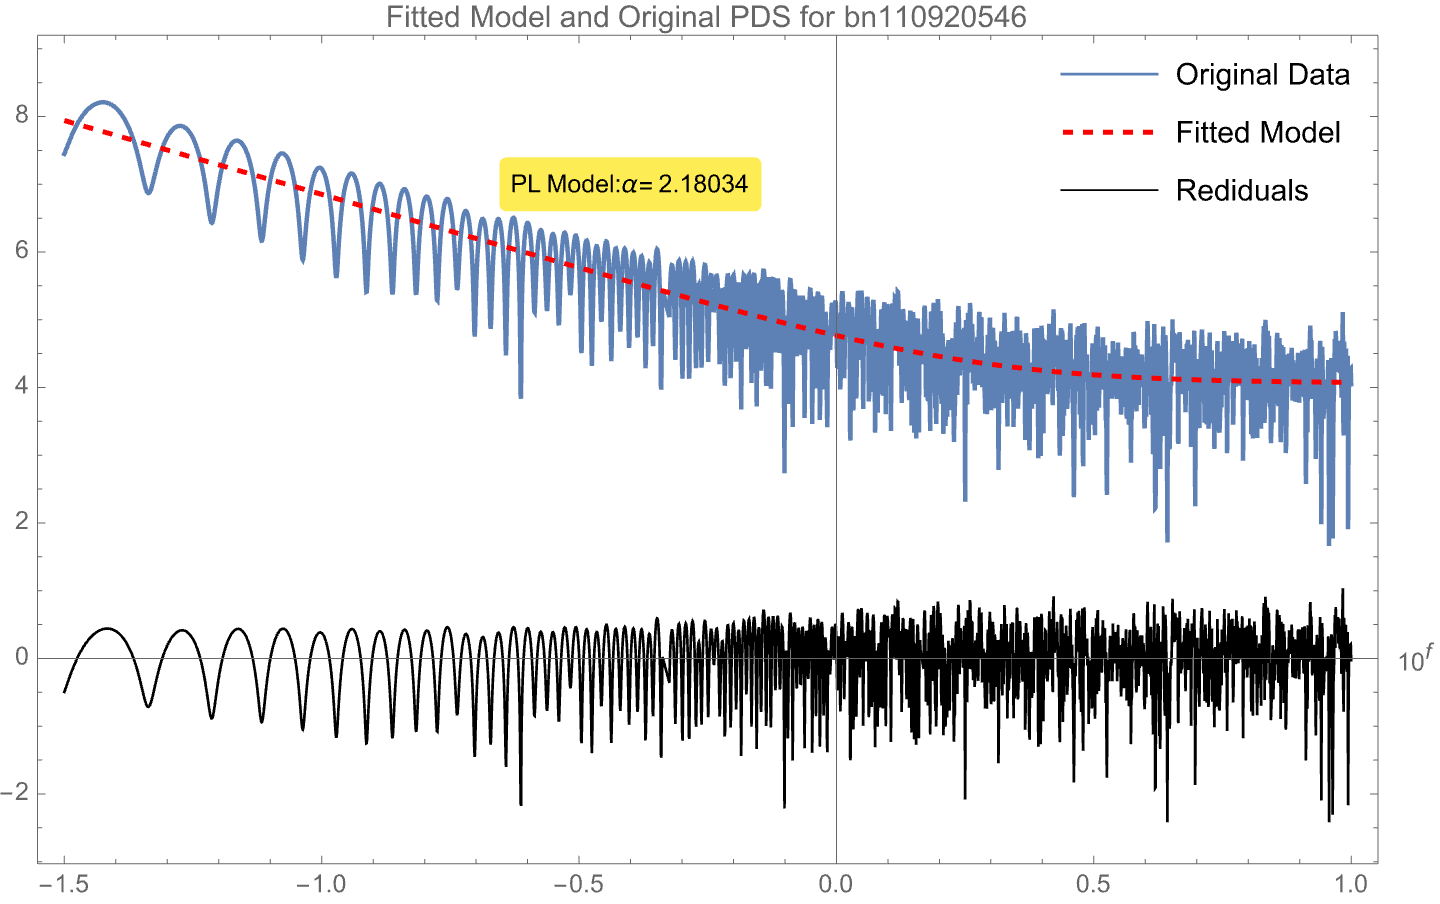
\includegraphics[width= 0.8\textwidth]{pds.png}
    \caption{\label{fig:pds.png}
        PDS curve of GRB 110920546.
    }
\end{figure}

(5) Model Fitting Module


From \cite{Dichiara:2016oob}, 

\newpage

\bibliography{pds}


\end{document}
